% !TEX root = ../thesis_main.tex
\chapter{Introduction}
%%%%%%%%%%%%%%%%%%%%%%%%%%%%%%%%%%%%%%%%%%%%%%%%%%%%%%
%  OPENING
%%%%%%%%%%%%%%%%%%%%%%%%%%%%%%%%%%%%%%%%%%%%%%%%%%%%%%
Humans can learn about new concepts and solve complex problems from limited, noisy or inconsistent observations and routinely make successful generalizations based on them, yet it remains a key challenge for machines to learn from such imperfect supervision. Most of today's success of data-driven machine learning systems depends on the availability of a massive amount of high-quality labeled data.

% detour to human learning
In the context of human learning, the argument of learning with imperfect supervision has been advanced under the name ``\emph{poverty of the stimulus}'', proposed by \citet{chomsky1980rules}. It suggests that human children can learn something as complex as a natural language from the limited inputs of variable quality and need no evidence for much of the knowledge they bring to the learning process. 
% how to explain human learning considering POS?
To explain this, some researchers postulate the innateness of some knowledge.
Along with this line, Chomsky noted~\citep{chomsky1980rules}:
\begin{quote}
    ``\emph{My own suspicion is that a central part of what we call “learning” is actually better understood as the growth of cognitive structures along an internally directed course under the triggering and partially shaping effect of the environment.}''
\end{quote}

% back to machine learning
Like humans, machines are confronted with the intriguing problem of the poverty of stimulus in learning and knowledge acquisition, although capturing such human-level learning abilities, given imperfect supervision, in machines remains a fundamental challenge in many domains~\citep{lake2017building}. 
%
% pos in machines and the necessity of {data-driven + innately primed} learning 
In machine learning, a similar discussion has been put forward on how learning algorithms can deal with the problem of \emph{poverty of stimulus}. It has been argued that a learner that makes no prior assumptions has no rational basis for generalizing over unseen instances~\citep{Mitchell:1997:ML}, which implies ``the futility of unbiased learning''.\footnote{There has been a long discussion between rationalists and empiricists in Philosophy and linguistics. Here, we just want to draw a connection between the process of learning in humans and machines in terms of \emph{poverty of stimulus}.}

%%%%%%%%%%%%%%%%%%%%%%%%%%%%%%%%%%%%%%%%%%%%%%%%%%%%%%
%  FIRST PART OF THE TITLE: "LEARNING WITH IMPERFECT SUPERVISION [...]"
%%%%%%%%%%%%%%%%%%%%%%%%%%%%%%%%%%%%%%%%%%%%%%%%%%%%%%
% What is important supervising and why learning with imperfect supervision?

The performance of machine learning models is often strongly correlated with the amount of available labeled data:
the more data you have, the more accurate your model will be~\citep{halevy2009unreasonable,sun2017revisiting}.  
However, in many real-world applications, large-scaled high-quality training data is not available.
This highlights the increasing need for building models with the ability to learn complex tasks with \emph{imperfect supervision}. 
In this thesis, we use ``\emph{imperfect supervision}'' as an umbrella term covering a variety of situations where the learning process is based on imperfect training samples~\citep{zhou2018brief}.


%%%%%%%%%%%%%%%%%%%%%%%%%%%%%%%%%%%%%%%%%%%%%%%%%%%%%%
%  SECOND PART OF THE TITLE: "[...] FOR LANGUAGE UNDERSTANDING"
%%%%%%%%%%%%%%%%%%%%%%%%%%%%%%%%%%%%%%%%%%%%%%%%%%%%%%
% why language understanding?
We focus on language understanding and reasoning as a pivotal problem in artificial intelligence.  Understanding language is one of the extraordinary cognitive abilities of humans. 
There have been several attempts to study whether non-human animals can acquire human language~\citep{pepperberg2017animal}, like Project Nim\footnote{\url{https://nl.wikipedia.org/wiki/Project_Nim}}, a research project that was mounted in the 1970s to determine whether a chimpanzee, named Nim Chimpsky, raised in close contact with humans could develop a limited language. 
Regardless of whether at the end of the project Nim was using language to communicate or simply going through a bag of tricks to get things, Nim's language was much more limited compared to what a human child can develop in the early years. 
%
This indicates that achieving human-level understanding and generation of language would not be an easy goal for machines either and despite the good performance on benchmark datasets, machines are nowhere near the skill of humans at language understanding and reasoning.

Here, in this thesis, we concentrate on language understanding and reasoning in more principled ways to improve the learning process than ad-hoc and domain or task-specific tricks to improve the output. We investigate our ideas on a wide range of sequence modeling and language understanding tasks.

%%%%%%%%%%%%%%%%%%%%%%%%%%%%%%%%%%%%%%%%%%%%%%%%%%%%%%
%  CLOSING THE INTRO SECTION IF THE INTRODUCTION CHAPTER!
%%%%%%%%%%%%%%%%%%%%%%%%%%%%%%%%%%%%%%%%%%%%%%%%%%%%%%
\medskip
% Although machine learning has made a lot of progress on mastering its practical shortcomings, e.g., modern neural networks overcoming the limitations of the early perceptrons~\citep{minsky69perceptrons}, some of the fundamental limitations, e.g., Chomsky's Poverty of Stimulus, remain.

The main problem we study in this thesis is the poverty of stimulus for learning algorithms and how to overcome this problem, we focus on  i) \emph{employing prior knowledge}, ii) \emph{augmenting data and learning to learn how to better use the data}, and iii) \emph{introducing inductive biases into learning algorithms}, all to improve the learning process. We believe these approaches are important ways to move toward better machine learning systems that are able to generalize over observed imperfect supervision signals. As \citet{Mitchell80theneed} already states in his paper:
\begin{quote}
``\emph{If biases and initial knowledge are at the heart of the ability to generalize beyond observed data, then efforts to study machine learning must focus on the combined use of prior knowledge, biases, and observation in guiding the learning process. It would be wise to make the biases and their use in controlling learning just as explicit as past research has made their observations and use.}''
\end{quote}

There are many domains and applications that suffer from the lack of a large amount of high quality labeled data, since it is not either possible or economically reasonable to build such training datasets. Building machine learning systems that can learn with imperfect supervision dramatically extends the scope where AI-powered systems can be applied, and more generally, contributes to the broader goal of democratizing AI.

\section{Problem Description and Research Questions}
Curating a large amount of high quality labeled training data has become the primary bottleneck in developing new methods and applications in machine learning~\citep{Ratner:2016}. 
% high-level ideas to deal with a lack of data
In practice, to deal with data scarcity in many tasks and applications, we can use higher-level approaches to provide supervision signals for training learning algorithms. 
% a list of alternative approaches
This can be done for instance by:
\begin{itemize}
\setlength\itemsep{0em}
\item 
Using distant, or heuristic supervision~\citep{Ratner:2016,Deriu2016:SemEval,Severyn:2015:SemEval, Dehghani:2016:SIGIR, dehghani:2018:ICLR, Dehghani:2017:nips_metalearn, Ratner:2016,Rekatsinas:2017,Varma:2017};
%
\item
Using incidental signals that exist in the data and the environment independently of the tasks and they are co-related to the target tasks~\citep{roth2017incidental}; 
%
\item
Introducing a form of structured prior knowledge~\citep{Dehghani:CIKM2016:long,Dehghani:2016:ICTIR};
%
\item
Exploiting noisy and inaccurate labels~\citep{Vahdat:2017, Lee:2013,Hinton:2015,Brodley:1999,reed2014training, Patrini:2016, patrini2016loss,malach2017decoupling,Ratner:2016};
%
\item
Using indirect supervision, like providing supervision by specifying constraints that should hold over the output space~\citep{stewart2017label, clarke2010driving};
%
\item
Applying bootstrapping, self-supervised feature learning, and data augmentation to make statistically efficient reuse of available data~\citep{cubuk2018autoaugment, miyato2018virtual, Qizhe:2019:uda, dosovitskiy2016discriminative,donahue2016adversarial};
%
\item
Using transfer learning to generalize knowledge across domains and tasks~\citep{Ruder:2019};
%
\item
Using active learning and response-based supervision in which the model receives feedback from interacting with an environment~\citep{clarke2010driving,riezler2014response};
%
\item
Zero/one/few-shot learning~\citep{vinyals2016matching,finn2017model,snell2017prototypical,socher2013zero};
%
\item
Injecting inductive biases into algorithms to generalize better on unobserved data~\citep{cohen2016group, cohen2016steerable, Dehghani:ICLR:2019}.
\end{itemize}

In a general supervised learning scenario, each training sample, which is used as the supervision signal, consist of a \emph{feature vector} (also called data instance) and a \emph{label}. However, in many domains and applications, there is an imperfection in the supervision signal. Here, in this thesis, we focus on two main problems: dealing with \emph{noisy} training data and dealing with \emph{limited} training data. 
We formulate the main research question that is addressed in this thesis as follows:
\resq{main}

Based on the above terminology, i.e., features versus label and noisy versus limited, we can presume different types of imperfections in the supervision signal. In each part of this thesis, we target one or some of these types and proposed ideas that can improve the learning process with that type of imperfection in supervision. 
Figure~\ref{fig:thesis_parts} summarizes the different types of imperfection of the supervision that we consider in each part of this thesis.\footnote{These combinations are the most common and rational cases in practical situations.}
\begin{figure}[t]
    \centering
    \begin{subfigure}[b]{0.32\textwidth}
    \centering
        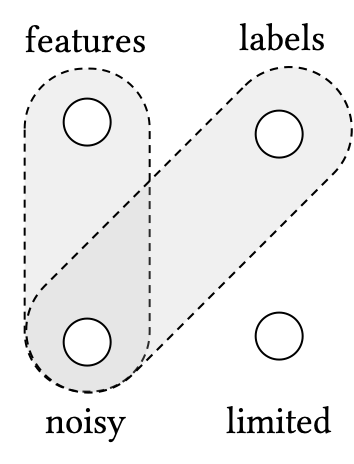
\includegraphics[width=0.55\linewidth]{01-introduction/figs_and_tables/fig_p1.png}
        \caption{\label{fig:p1}Part I}
    \end{subfigure}
        ~ 
    \begin{subfigure}[b]{0.32\textwidth}
    \centering
        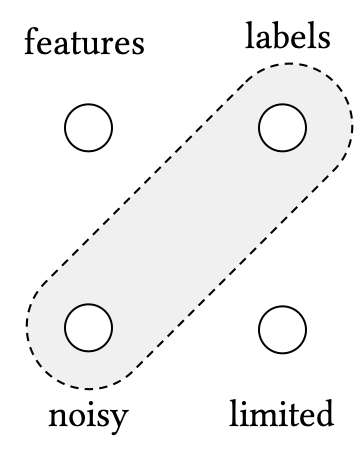
\includegraphics[width=0.55\linewidth]{01-introduction/figs_and_tables/fig_p2.png}
        \caption{\label{fig:p2}Part II}
    \end{subfigure}
        ~ 
    \begin{subfigure}[b]{0.32\textwidth}
    \centering
        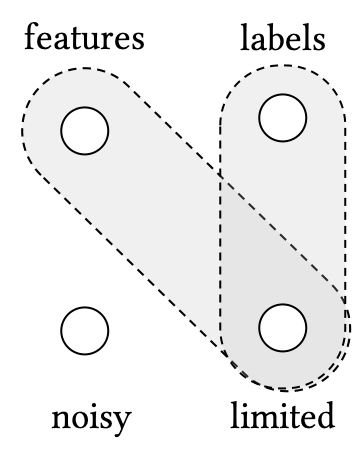
\includegraphics[width=0.55\linewidth]{01-introduction/figs_and_tables/fig_p3.png}
        \caption{\label{fig:p3}Part III}
    \end{subfigure}
\caption{\label{fig:thesis_parts}Different types of imperfection in the supervision that we deal with in each part of this thesis.}
\end{figure}

\bigskip
In Part~\ref{part1} of the thesis, we address the problem of noisy features. We propose robust models that can deal with non-relevant terms in relevant documents when modeling the notion of relevance in the context of relevance feedback tasks for document ranking. We also propose models that are capable of detecting and ignoring the unstable features that change over time when learning representations from data that evolves over time, as noisy factors in the data. We also partly address the problems of noisy labels by modeling the relevance in pseudo-relevance feedback tasks for document ranking, where top-k ranked documents in a retrieval run are assumed as relevant documents, while this assumption does not hold for all cases.

The proposed models in Part~\ref{part1} organized around the idea of exploring how the structure of the data can be incorporated as prior knowledge to learn representations that are more robust against noise and changes in the data over the time. 
The following research question is the main question is central to Part~\ref{part1} of the thesis:
\resq{p1}

\bigskip
In Part~\ref{part2} of the thesis, we target the problem of noisy or weak labels. We study how we can develop neural networks that can learn from weakly annotated training samples with the ability to go beyond the imperfection of the weak labels. We study different architectural choices and objective functions for neural ranking models to find a more noise tolerant model when learning from pseudo-labels.  We also introduce ideas that meta-learn the fidelity of weakly annotated labels and modulate the learning process based on the fidelity scores of weakly labeled samples. In fact, in this part, we make assumptions in the act of observing the data, like how to select the data based on the fidelity of data points, which is also a form of incorporating knowledge and biases.
In this part, we address the following research question:
\resq{p2}

\bigskip
In Part~\ref{part3}, we deal with the problem of limited labeled data, for instance, in the context of bAbI reasoning tasks with 1k training samples where the tasks are complex and training data is limited. We also study the cases where we have a lot of labeled samples, but with limited coverage, which can be seen as the limitation in the diversity of feature vectors. For instance in the context of algorithmic tasks, with the intention of assessing the ability of models on length generalization, we have plenty of training data but the distribution of sample's length in training is different from the test set. 
In this part, we investigate the idea of injecting some inductive biases\footnote{Inductive biases are ``any biases for choosing one generalization over another, other than strict consistency with the observed training samples.'' as defined by~\citet{Mitchell80theneed}. We elaborate on this at the beginning of Part~\ref{part3}.} into models in order to encode modeling assumptions that help the models to be more data efficient and generalize better.
The main research question that is addressed in Part~\ref{part3} is:
\resq{p3}


\subsection{Language Understanding and Sequence Modeling Tasks}
We study our research questions in the context of sequence modeling and natural language understanding, generation, and reasoning tasks. In the course of this thesis, we cover a wide range of tasks, including:
\begin{itemize}
\item 
Assessing relevance for ranking (Chapter~\ref{chap:2}, \ref{chap:4}, \ref{chap:5});
%
\item 
(Pseudo)-relevance feedback for document ranking(Chapter~\ref{chap:2});
%
\item 
Contextual suggestion and recommendation~\citep{hashemioverview} (Chapter~\ref{chap:2});
%
\item 
Text classification (over time)~\citep{Hirst:2014} (Chapter~\ref{chap:3});
%
\item 
Sentiment analysis~\citep{rosenthal2017semeval, Nakov:2016, rosenthal:2015} (Chapter~\ref{chap:5}); 
%
\item 
Machine Translation (Chapter~\ref{chap:6});
%
\item 
Natural language reasoning ---bAbI tasks~\citep{weston2015towards} (Chapter~\ref{chap:6});
%
\item 
Broad context language modeling~\citep{paperno2016lambada} (Chapter~\ref{chap:6});
%
\item 
Open-domain question answering~\citep{dunn2017searchqa, dhingra2017quasar} (Chapter~\ref{chap:6});
%
\item 
Modeling the structure in natural language sentences---subject-verb agreement task~\citep{linzen2016assessing} (Chapter~\ref{chap:6});
%
\item 
Learning to execute computer programs~\citep{ZS14} (Chapter~\ref{chap:6}); 
%
\item 
Algorithmic problems, like arithmetic and sequence memorization tasks ~\citep{neural_gpu} (Chapter~\ref{chap:6}).
\end{itemize}

Besides the challenges of learning from imperfect supervision in many of these tasks, some of them are difficult tasks that, for instance, require learning rich representations, or capturing complex underlying relations, or detecting and understanding abstract concepts and reasoning about them.
%
Although we mainly focus on sequence modeling and language-related tasks and evaluate our proposed ideas on these tasks, many of the proposed algorithms in this thesis can be easily extended to other domains like computer vision.
%

In the next section, we present an overview of the thesis and introduce the structure of the content and summarize different chapters in each part of the thesis.

\section{Thesis Overview}
This thesis consists of the introductory matter, followed by five main
chapters that are divided into three parts that are described in the previous section.~\footnote{This thesis consists of papers that contribute to the field of information retrieval, natural language processing, and machine learning, thus the terminology used in different parts might change accordingly.} Finally, it closes off with the Conclusions and Bibliography. 

\subsection*{PART I: \titleof{p1}}
In this part, we explore how taking the general structured of the data into account can help to estimate representations that capture only the significant features when the data is noisy and highly variant over time. We break our discussions in this part of the thesis into two chapters:

\subsubsection*{Chapter 2: \titleof{c2}}
In this chapter, we address the following research question:
\resq{c2}
We introduce \emph{\swlms} (\acswlm)~\citep{Dehghani:2016:SIGIR} to learn a representation for a set of textual entities, where this representation captures all, and only, the \textit{significant} shared features from these entities.  \acswlm adjusts the weights of features to decrease the weight of noisy terms that are either well explained by all the entities, i.e., too general or only explained by a specific entity in the set, i.e., too specific, which eventually results in having the significant features left in the model.  
We employ \acswlm in two language understanding tasks: the feedback problem in document ranking~\citep{Dehghani:CIKM2016:long, Dehghani:CIKM2016:short}, and group profiling in content personalization and recommendation tasks~\citep{Dehghani:2016:CHIIR,Dehghani2016:trec}. We show how \acswlm is remarkably robust against noisy features like non-relevant terms in relevant documents in the feedback task. 

\subsubsection*{Chapter 3: \titleof{c3}}
In this chapter, we address the following research question:
\resq{c3}
We extend \emph{\swlms} to hierarchically structured data and introduce \emph{\hswlms} (\achswlm)~\citep{Dehghani:2016:ICTIR, Dehghani:2016:CLEF} which is an iterative approach that learns representations for hierarchical entities that are highly separable as \acswlm removes the features that are well explained by either the ancestors (general features) or individual descendants (specific features). In this chapter, we discuss what makes separability a desirable property for classifiers and show how obtaining this property increases the robustness of representations against the structural changes in the data during the time.

\subsection*{PART II: \titleof{p2}}
In this part, we study how we can supervise machine learning systems by labeling training data programmatically instead of labeling by hand and discuss how to design neural networks that learn to go beyond the imperfection in the weakly annotated data. We break this into two chapters:

\subsubsection*{Chapter 4: \titleof{c4}}
In this chapter, we address the following research question:
\resq{c4}
In this chapter, we propose to train a neural ranking model using weak labels that are obtained automatically without human annotators or any external resources (e.g., click data). We train a set of simple yet effective neural ranking models and study their effectiveness under various learning scenarios, i.e., point-wise and pair-wise, different objective functions, and using different input representations~\citep{Dehghani:2017:SIGIR}. We also discuss how privacy preserving approaches can benefit from models that are capable of learning from weak signals, where instead of labels from the original sensitive training data a noisy version is provided~\citep{dehghani:2017:neuir}.

\subsubsection*{Chapter 5: \titleof{c5}}
In this chapter, we focus on the following research question:
\resq{c5}

In this chapter we introduce \emph{Learning with Controlled Weak Supervision (\cws)} and \emph{Fidelity Weighted Learning (\fwl)}, two semi-supervised approaches for training neural networks, where we have a large set of data with weak labels and a small amount of data with true labels. 
%
In \cws we train two neural networks in a meta-learning setup: a \tnet, the learner, and a \cnet, the meta-learner.  The \tnet is optimized to perform a given task and is trained using a large set of unlabeled data that are weakly annotated. We propose to control the magnitude of the gradient updates to the \tnet using the scores provided by the second \cnet, which is trained on a small amount of supervised data. Thus we avoid that the weight updates computed from noisy labels harm the quality of the \tnet model.

\fwl is a student-teacher approach in which we modulate the parameter updates to a \emph{student} network (trained on the task we care about) on a per-sample basis according to the posterior confidence of its label-quality estimated by a \emph{teacher} (who has access to the high-quality labels).  

\subsection*{PART III: \titleof{p3}}
In this part, we discuss injecting inductive biases into learning algorithms as a way to help them to come up with more generalizable solutions when they are provided with limited observations. We further discuss how we can improve the generalization of Transformers~\citep{transformer}, the self-attentive feed-forward networks for sequence modeling, by introducing a recurrent inductive bias into their architecture.

\subsubsection*{Chapter 6: \titleof{c6}}
In this chapter, we address the following research question:
\resq{c6}
We introduced Universal Transformer~\citep{Dehghani:ICLR:2019}, a self-attentive concurrent-recurrent sequence model, which is an extension of the Transformer model~\citep{vaswani2017attention}. The Universal Transformer introduces recurrence in depth by repeatedly modifying a series of vector representations for each position of the sequence in parallel, by combining information from different positions using self-attention and applying a recurrent transition function across all time steps. 
In the simplest form, a Universal Transformer with a fixed number of iterations is almost equivalent to a multi-layer Transformer with tied parameters across all its layers. By sharing weights, we can save massively on the number of parameters that we are training and fewer parameters means that we learn faster with fewer data points.  We show that the elegant idea of introducing recurrence in depth enables the Universal Transformer to extrapolate from training data much better on a range of algorithmic and language understanding tasks~\citep{Dehghani:ICLR:2019, Dehghani:2019:WSDM}.

\bigskip
While the three parts of the thesis offer a complete story aligned with the goal of \emph{improving the learning process by incorporating prior knowledge, introducing right biases, and making best use of the observations from the data}, they can be read independently. 
Each of the chapters of the thesis also has their own independent research questions, proposed ideas, and take home messages, but we recommend reading them with the order they appeared in the parts.


\section{Origins}
Next, we present the origins of each chapter in terms of the papers they are based on.
\begin{itemize}
    \setlength{\itemindent}{-28pt}
    \item[]\textbf{Part I:} \emph{\titleof{p1}}
%  
        \begin{itemize}
            \setlength{\itemindent}{-33pt}
            \item[]\textbf{Chapter 2:} \emph{\titleof{c2}}
            \begin{itemize}[label=\textbullet] 
                \item \bibentry{Dehghani:CIKM2016:long}.
                \item \bibentry{Dehghani:2016:CHIIR}.
                \item \bibentry{Dehghani2016:trec}.
                \item \bibentry{Dehghani:2016:SIGIR} (SIGIR Doctoral Consortium Award).
            \end{itemize}
            
            {\footnotesize{MD designed the models, implemented the algorithms, ran the experiments, and did most of the writing. HA helped with the implementation and experiments. JK and DH helped with designing the model. HA, JK, DH, and MM contributed to the writing.}\medskip}
            
    
            \item[]\textbf{Chapter 3:} \emph{\titleof{c3}}
            \begin{itemize}[label=\textbullet] 
                \item \bibentry{Dehghani:2016:ICTIR} (Best Paper Award).
                \item \bibentry{Dehghani:2016:CLEF} (Best Paper Honorable Mention).
            \end{itemize}
            {\footnotesize{MD designed the models, implemented the algorithms, ran the experiments, and did most of the writing. HA helped with the implementation and experiments. JK helped with designing the model. HA, JK, and MM contributed to the the writing.}\medskip}
        \end{itemize}
%  
% \end{itemize}
% \begin{itemize}
% \setlength{\itemindent}{10pt}
    \item[] \textbf{Part II:} \emph{\titleof{p2}}
%  
        \begin{itemize}
            \setlength{\itemindent}{-33pt}
            \item[] \textbf{Chapter 4:} \emph{\titleof{c4}}
            \begin{itemize}[label=\textbullet] 
                \item \bibentry{Dehghani:2017:SIGIR}.
                \item \bibentry{dehghani:2017:neuir}.
                \item \bibentry{Dehghani2017:CIKM}.
            \end{itemize}
            {\footnotesize{MD designed the models, implemented the algorithms, ran the experiments, and did most of the writing. 
            SR and HZ helped with designing the models. SR helped with the implementation. HZ, HA, AS, SR, and JK helped with designing the experiments. EA and PF mentored the (internship) project. HZ, HA, JK, BC, MdR, SR, AS, and PF helped with writing.}\medskip}
                        
            \item[] \textbf{Chapter 5:} \emph{\titleof{c5}}
            \begin{itemize}[label=\textbullet] 
                \item \bibentry{dehghani:2018:ICLR}.
                \item \bibentry{Dehghani:2017:nips_metalearn}.
                \item \bibentry{Dehghani:2017avoiding}.
            \end{itemize}
            {\footnotesize{MD designed the models, implemented the algorithms, ran the experiments, and did most of the writing. 
            AM helped with designing the models. AM, SG, JK, and AS helped with designing the experiments. AM, SG, AS, SR, JK, and BS helped with writing.}\medskip}
        \end{itemize}
%   
% \end{itemize}
% \begin{itemize}
% \setlength{\itemindent}{10pt}
    \item[] \textbf{Part III:} \emph{\titleof{p3}}
%  
        \begin{itemize}
            \setlength{\itemindent}{-33pt}
            \item[] \textbf{Chapter 6:} \emph{\titleof{c6}}
            \begin{itemize}[label=\textbullet] 
                \item \bibentry{Dehghani:ICLR:2019}.
                \item \bibentry{Dehghani:2019:WSDM}.
            \end{itemize}
        \end{itemize}
        {\footnotesize{MD co-designed the core model (first paper) with SG, and MD extend the model (second paper). MD implemented the algorithms, ran all the experiments, and helped with the writing. SG and OV mentored the (internship) project. SG led the writing. OV, JU, and LK helped with designing the model and designing the experiments. OV, JU, LK, HA, JK, and MdR helped with the writing.}\medskip}
%
\end{itemize}

The thesis also indirectly builds on the following papers (listed in reverse chronological order):
%  
\begin{itemize}
    \item \bibentry{Dehghani:2019:ICLR-LLD}.
    \item \bibentry{Dehghani:2018:SIGIRForum}.
    \item \bibentry{Zamani:2018:CIKM}.
    \item \bibentry{Azarbonyad:2018:TKDE}.
    \item \bibentry{Dehghani:2018:LND4IR}.
    \item \bibentry{Zamani:2018:LND4IR}.
    \item \bibentry{Azarbonyad:2017:CIKM}.
    \item \bibentry{Kenter:2017:NN4IR}.
    \item \bibentry{Dehghani:2017:ICTIR}.
    \item \bibentry{Dehghani:2017:CHIIR}.
    \item \bibentry{Dehghani:2017:CHIIR}.
    \item \bibentry{Azarbonyad:2017:ECIR}.
    \item \bibentry{Dehghani:2016:DIR}.
    \item \bibentry{Dehghani:CIKM2016:short}.
    \item \bibentry{Quiroz:2016:CLEF}.
    \item \bibentry{Hashemi:2015:TREC}.
    \item \bibentry{Dehghani:2015:DIR}.
    \item \bibentry{Tabrizi:2015:ICTIR}.
    \item \bibentry{Azarbonyad:2015:CLEF}.
    \item \bibentry{Azarbonyad:2015:SIGIR}.
    \item \bibentry{Dehghani:2015:ECIR}.
    \item \bibentry{Olieman:2014:ERD}
\end{itemize}